%*******10********20********30********40********50********60********70********80
%% ----------------------------------------------------------------
%% Thesis.tex -- MAIN FILE (the one that you compile with LaTeX)
%% ---------------------------------------------------------------- 

%% This template is based on Graduate Thesis written by Sunil Patel,
% (who based it on the ecsthesis template) under the LaTeX Project Public License.
% which can be found here: http://latex-project.org/lppl/
% in the hope that it will be easier to use and to scale down to your needs
% by Simon Ternsjö in 2013-10



% INSTRUCTIONS:

% The meaning is not to edit this document much, but to fill in information 
% in the different files in the folders;
% Settings, Frontpages, Chapters, Appendices and possibly Files,
% as well as the file Bibliography.bib

% This template is easy to scale down to suit your need, 
% simply comment the input statements explained below


% Set up the document:
\documentclass[a4paper, 11pt, oneside]{Thesis}  % Use the "Thesis" style, based on the ECS Thesis style by Steve Gunn

% Add more package in Package.tex:
% begin Appendix

\appendix
\chapter{Complete Set of Gathered Data}
\label{appendix-CompleteSetOfData}

\paragraph{ } The fields that are highlighted in the tables are unauthorized stops at which the buses picked up or dropped off passengers.

\begin{enumerate}

\item Trip Number: 2
\begin{itemize}
\item Date: 23/5/2013
\item Departure Time: 17.00pm
\item Departure Place: Kolpetty
\item Table~\ref{table-trip2-BoardingAndAlighting} and~\ref{table-trip2-LoiterTime}
\end{itemize}

\item Trip Number: 3
\begin{itemize}
\item Date: 23/5/2013
\item Departure Time: 18.14pm
\item Departure Place: Kolpetty
\item Table~\ref{table-trip3-BoardingAndAlighting} and~\ref{table-trip3-LoiterTime}
\end{itemize}

\item Trip Number: 4
\begin{itemize}
\item Date: 23/5/2013
\item Departure Time: 16.28pm
\item Departure Place: Rajagiriya
\item Table~\ref{table-trip4-BoardingAndAlighting} and~\ref{table-trip4-LoiterTime}
\end{itemize}

\item Trip Number: 5
\begin{itemize}
\item Date: 23/5/2013
\item Departure Time: 17.43pm
\item Departure Place: Rajagiriya
\item Table~\ref{table-trip5-BoardingAndAlighting} and~\ref{table-trip5-LoiterTime}
\end{itemize}

\end{enumerate}

%data tables

\begin{table}
\centering
\begin{tabular}{|l|r|r|r|r|}
\hline
Bus Stop & Boarded & Alighted & Net Gain & On Board \\
\hline
 & & & & 0 \\
Kolpetty Depot	&21	&0	&21	&21\\
Supermarket	&7	&1	&6	&27\\
Alwis Place	&5	&0	&5	&32\\
\rowcolor[gray]{0.7}
Citibank	&2	&0	&2	&34\\
Library	&7	&2	&5	&39\\
SLTA	&0	&1	&-1	&38\\
Nelum Pokuna	&3	&0	&3	&41\\
\rowcolor[gray]{0.7}
Alexandra Roundabout	&3	&0	&3	&44\\
\rowcolor[gray]{0.7}
Saudi Embassy	&1	&0	&1	&45\\
Asha Central	&6	&0	&6	&51\\
Wijerama	&0	&0	&0	&51\\
Borella	&9	&2	&7	&58\\
Devi Balika	&5	&0	&5	&63\\
Castle Street	&0	&0	&0	&63\\
Ayurveda	&0	&9	&-9	&54\\
Rajagiriya	&11	&7	&4	&58\\
\hline
\end{tabular}
\caption{Boarding And Alighting data for Trip 2}
\label{table-trip2-BoardingAndAlighting}
\end{table}

\begin{table}
\centering
\begin{tabular}{|l|r|r|r|}
\hline
Bus Stop & Arrival Time (h) & Departure Time (h) & Loiter Time (mins) \\
\hline
Kolpetty Depot	&	&17.03	&0\\
Supermarket	&17.03	&17.04	&1\\
Alwis Place	&17.05	&17.05	&0\\
Library	&17.08	&17.08	&0\\
SLTA	&17.09	&17.09	&0\\
Nelum Pokuna	&17.11	&17.12	&1\\
Asha Central	&17.15	&17.16	&1\\
Wijerama	&17.17	&17.18	&1\\
Borella	&17.21	&17.25	&4\\
Devi Balika	&17.27	&17.27	&0\\
Castle Street	&17.29	&17.29	&0\\
Ayurveda	&17.31	&17.38	&7\\
Rajagiriya	&17.40	&17.43	&3\\
\hline
Total Loiter Time & & & 18 mins \\
Duration of Trip & & 40 mins & \\
\hline
\end{tabular}
\caption{Loiter Time Data for Trip 2}
\label{table-trip2-LoiterTime}
\end{table}

\begin{table}
\centering
\begin{tabular}{|l|r|r|r|r|}
\hline
Bus Stop & Boarded & Alighted & Net Gain & On Board \\
\hline
 & & & & 0 \\
Kolpetty Depot	&37	&0	&37	&37\\
Supermarket	&10	&0	&10	&47\\
Alwis Place	&1	&0	&1	&48\\
Library	&4	&3	&1	&49\\
SLTA	&1	&0	&1	&50\\
\rowcolor[gray]{0.7}
Museum	&2	&0	&2	&52\\
Nelum Pokuna	&5	&2	&3	&55\\
Saudi Embassy	&0	&0	&0	&55\\
Asha Central	&3	&1	&2	&57\\
Wijerama	&0	&0	&0	&57\\
Borella	&10	&6	&4	&61\\
Devi Balika	&1	&0	&1	&62\\
Castle Street	&6	&2	&4	&66\\
Ayurveda	&3	&5	&-2	&64\\
Rajagiriya	&18	&12	&6	&70\\
\hline
\end{tabular}
\caption{Boarding And Alighting data for Trip 3}
\label{table-trip3-BoardingAndAlighting}
\end{table}

\begin{table}
\centering
\begin{tabular}{|l|r|r|r|}
\hline
Bus Stop & Arrival Time (h) & Departure Time (h) & Loiter Time (mins) \\
\hline
Kolpetty Depot	&	&18.19	&0\\
Supermarket	&18.20	&18.22	&2\\
Alwis Place	&18.23	&18.24	&1\\
Library	&18.26	&18.26	&0\\
SLTA	&18.28	&18.28	&0\\
Nelum Pokuna	&18.30	&18.30	&0\\
Asha Central	&18.35	&18.35	&0\\
Wijerama	&18.35	&18.35	&0\\
Borella	&18.37	&18.38	&1\\
Devi Balika	&18.41	&18.41	&0\\
Castle Street	&18.43	&18.43	&0\\
Ayurveda	&18.45	&18.45	&0\\
Rajagiriya	&18.47	&18.53	&6\\
\hline
Total Loiter Time & & & 10 mins \\
Duration of Trip & & 34 mins & \\
\hline
\end{tabular}
\caption{Loiter Time Data for Trip 3}
\label{table-trip3-LoiterTime}
\end{table}

\begin{table}
\centering
\begin{tabular}{|l|r|r|r|r|}
\hline
Bus Stop & Boarded & Alighted & Net Gain & On Board \\
\hline
 & & & & 19 \\
Rajagiriya	&15	&1	&14	&33\\
Cotta Road	&2	&0	&2	&35\\
Ayurveda	&4	&3	&1	&36\\
Castle Street	&3	&1	&2	&38\\
Borella	&2	&3	&-1	&37\\
Horton Place	&2	&2	&0	&37\\
Wijerama	&0	&2	&-2	&35\\
Asha Central	&7	&0	&7	&42\\
Nelum Pokuna	&2	&4	&-2	&40\\
Library	&19	&0	&19	&59\\
Liberty	&2	&16	&-14	&45\\
Galle Road	&0	&1	&-1	&44\\
\rowcolor[gray]{0.7}
St. Anthony's Mw	&1	&2	&-1	&43\\
Kolpetty Depot	&0	&43	&-43	&0\\
\hline
\end{tabular}
\caption{Boarding And Alighting data for Trip 4}
\label{table-trip4-BoardingAndAlighting}
\end{table}

\begin{table}
\centering
\begin{tabular}{|l|r|r|r|}
\hline
Bus Stop & Arrival Time (h) & Departure Time (h) & Loiter Time (mins) \\
\hline
Rajagiriya	&16.28	&16.33	&5\\
Cotta road	&16.34	&16.34	&0\\
Ayurveda	&16.35	&16.36	&1\\
Castle street	&16.38	&16.39	&1\\
Borella	&16.40	&16.41	&1\\
Horton Place	&16.42	&16.42	&0\\
Wijerama	&16.44	&16.44	&0\\
Asha Central	&16.47	&16.47	&0\\
Nelum Pokuna	&16.48	&16.48	&0\\
Library	&16.50	&16.50	&0\\
Liberty	&16.52	&16.52	&0\\
Galle Road	&16.54	&16.54	&0\\
Kolpetty Depot	&16.55	&	&0\\
\hline
Total Loiter Time & & & 8 mins \\
Duration of Trip & & 22 mins & \\
\hline
\end{tabular}
\caption{Loiter Time Data for Trip 4}
\label{table-trip4-LoiterTime}
\end{table}

\begin{table}
\centering
\begin{tabular}{|l|r|r|r|r|}
\hline
Bus Stop & Boarded & Alighted & Net Gain & On Board \\
\hline
 & & & & 30 \\
Rajagiriya	&5	&2	&3	&33\\
Cotta Road	&2	&0	&2	&35\\
Ayurveda	&0	&4	&-4	&31\\
Castle Street	&2	&0	&2	&33\\
Borella	&1	&6	&-5	&28\\
Horton Place	&3	&2	&1	&29\\
\rowcolor[gray]{0.7}
Chatz	&1	&0	&1	&30\\
Wijerama	&1	&0	&1	&31\\
Asha Central	&1	&1	&0	&31\\
Nelum Pokuna	&5	&3	&2	&33\\
Library	&4	&3	&1	&34\\
Liberty	&0	&8	&-8	&26\\
Galle Road	&0	&4	&-4	&22\\
\rowcolor[gray]{0.7}
St. Anthony's Mw	&4	&3	&1	&23\\
Kolpetty Depot	&0	&23	&-23	&0\\
\hline
\end{tabular}
\caption{Boarding And Alighting data for Trip 5}
\label{table-trip5-BoardingAndAlighting}
\end{table}

\begin{table}
\centering
\begin{tabular}{|l|r|r|r|}
\hline
Bus Stop & Arrival Time (h) & Departure Time (h) & Loiter Time (mins) \\
\hline
Rajagiriya	&17.40	&17.43	&3\\
Cotta Road	&17.44	&17.45	&1\\
Ayurveda	&17.49	&17.49	&0\\
Castle Street	&17.52	&17.52	&0\\
Borella	&17.55	&17.56	&1\\
Horton Place	&17.57	&17.58	&1\\
Wijerama	&17.59	&17.59	&0\\
Asha Central	&18.00	&18.00	&0\\
Nelum Pokuna	&18.01	&18.02	&1\\
Library	&18.03	&18.03	&0\\
Liberty	&18.05	&18.05	&0\\
Galle Road	&18.08	&18.08	&0\\
Kolpetty Depot	&18.09	&	&0\\
\hline
Total Loiter Time & & & 7 mins \\
Duration of Trip & & 26 mins & \\
\hline
\end{tabular}
\caption{Loiter Time Data for Trip 5}
\label{table-trip5-LoiterTime}
\end{table}

% Use if you want:
%5%\graphicspath{Figures/}  % Location of the graphics files (set up for graphics to be in PDF format)
%5%\hypersetup{urlcolor=blue, colorlinks=true}  % Colours hyperlinks in blue, but this can be distracting if there are many links.

% Set your name, the title of the report and more in Administrative.tex:
% This is where author, university, title and more is defined

% Personal information:
\newcommand{\myAuthorName}  {Hanna Abbott}% Author Name
\newcommand{\myAuthorEmail} {hanna.abbott@hogwarts.se} % Author email
\newcommand{\myTitle}       {The properties of Moonstone and its uses in Potion making} % Thesis title goes here
\newcommand{\mySubject}     {Potions} % Subject goes here
\newcommand{\myKeywords}    {Moonstone, Potion, Drafts, Magical} % Keywords goes hear




% University information
\newcommand{\myUniversity}{Hogwarts} %The Iniversity name goes here
\newcommand{\myUniversityWeb}{http://www.jkrowling.com/} %University Web Site URL Here (include http://
\newcommand{\myDepartment}{Department of Hufflepuff} % The Department goes here 
\newcommand{\myDepartmentWeb}{http://www.harrypotterwizardscollection.com/} % Department Web Site URL Here (include http://)
\newcommand{\myGroup}{Research Group Name}
\newcommand{\myGroupWeb}{Research Group Web Site URL Here (include http://)}
\newcommand{\myFaculty}{Faculty of ...}
\newcommand{\myFacultyWeb}{Faculty Web Site URL Here (include http://)}

%Degree, program or corse: ex: Master of Science, Engineering Physics
\newcommand{\myDegree}{Ordinary Wizarding Level} % The degree, program or course-name goes here


% can be left untouched, both:
\newcommand{\myDate}{\today}
\newcommand{\myPartyalFulfillment}{A thesis submitted in partial fulfillment for the degree of}

%% ----------------------------------------------------------------
\begin{document}
\frontmatter      % Begin Roman style (i, ii, iii, iv...) page numbering


% Here the first pages are imported, you can find them in the Frontpages folder
% Files in the subfolder Fixed does not need to be edited.
% If you don't need any of these sections, simply comment, or delete, the input-row


%% All the pages before the chapters ------------------------------
% Set up the Title Page - DO NOT EDIT THIS, (if you don't want to ;)  )
% instead specify your name, title and more in "/Settings/Administrative.tex"
\title   {\myTitle}
\authors {\texorpdfstring
            {\href{\myAuthorEmail}{\myAuthorName}}
            {\myAuthorName}
         }
\addresses  {\groupname\\\deptname\\\univname}  
\date       {\myDate}
\subject    {\mySubject}
\keywords   {\myKeywords}

\maketitle
%% ----------------------------------------------------------------

\setstretch{1.3}  % It is better to have smaller font and larger line spacing than the other way round

% Define the page headers using the FancyHdr package and set up for one-sided printing
\fancyhead{}  % Clears all page headers and footers
\rhead{\thepage}  % Sets the right side header to show the page number
\lhead{}  % Clears the left side page header


%% ----------------------------------------------------------------
% Declaration Page required for the Thesis, your institution may give you a different text to place here
\pagestyle{fancy}  % Finally, implement the FancyHdr headers
\clearpage
\Declaration{

\addtocontents{toc}{\vspace{1em}}  % Add a gap in the Contents, for aesthetics

I, \myAuthorName, declare that this thesis titled, `\myTitle' and the work presented in it are my own. I confirm that:

\begin{itemize} 
\item[\tiny{$\blacksquare$}] This work was done wholly or mainly while in candidature for a research degree at this University.
 
\item[\tiny{$\blacksquare$}] Where any part of this thesis has previously been submitted for a degree or any other qualification at this University or any other institution, this has been clearly stated.
 
\item[\tiny{$\blacksquare$}] Where I have consulted the published work of others, this is always clearly attributed.
 
\item[\tiny{$\blacksquare$}] Where I have quoted from the work of others, the source is always given. With the exception of such quotations, this thesis is entirely my own work.
 
\item[\tiny{$\blacksquare$}] I have acknowledged all main sources of help.
 
\item[\tiny{$\blacksquare$}] Where the thesis is based on work done by myself jointly with others, I have made clear exactly what was done by others and what I have contributed myself.

\end{itemize}
 
\vspace{10 mm}
 
Signed:\\
\rule[1em]{25em}{0.5pt}  % This prints a line for the signature

Date:\\
\rule[1em]{25em}{0.5pt}  % This prints a line to write the date
}



% The "Funny Quote Page"
\clearpage
\pagestyle{empty}  % No headers or footers for the following pages

%use 1 or vfill to position the quote where it looks good:
\null\vfill\vfill


% Now comes the "Funny Quote", written in italics:

\textit{
    % Write a funny quote here:
    ''We did it, we bashed them, wee Potter’s the one, \\
    and Voldy’s gone moldy, so now let’s have fun!''
}
\begin{flushright}
    % If the quote is taken from someone, their name goes here:
    - Peeves
\end{flushright}


 
\vfill\vfill\vfill\vfill\vfill\null


% begin Abstract
\clearpage
\chapter*{Abstract}

\paragraph{ } The Private Bus Passenger Transportation System is the most widely used Public Transportation System in Sri Lanka. It is used as the primary transport method for passengers within Colombo, the most populous city in the country, as well as between Colombo and other cities as well as suburbs.

However, the system is rife with inefficiencies and shortcomings. Delays, overcrowded buses and bus strikes are commonplace and the service is of poor quality. The problems in the system do not merely affect the transportation industry but has a knock-on effect to all walks of daily life for the people in the country. The productivity of the workforce suffers due to this inefficiency in the main public transport system.

The biggest problem that the commuters outline is the need to improve the service in terms of its schedule reliability and passenger overcrowding. Meanwhile, the bus operators complain that the revenue leakage is a major issue and needs to be rectified. However, the status quo continues without any solutions and these problems continue to haunt the average commuter.

Research into the issues as well as comments from frequent commuters has shown that the underlying cause is the lack of a proper Information System to assist the stakeholders in their decision making processes. Therefore, this research analyses the problems prevalent in the system and provides a solution to help minimize/eliminate the existing problems. The project identifies key aspects in the solution prototype and generalizes the results so that the concept can be applied to other developing countries with similar environments.


% begin Acknowledgement
\clearpage
\chapter*{Acknowledgement}
I would like to take this opportunity to thank the following people who have helped me thus far in my final year research project.
\begin{itemize}
\item Dr. Shiromi Arunatilake, for acting as my supervisor, overseeing my work and giving her valuable input into the thinking process of the project.
\item Dr. Jeewani Goonathilake, for providing her assistance whenever possible in her capacity as the Course Coordinator for the \acrshort{ict} Research Projects.
\item Mr. Pradeep Fernando, the Head of the \acrshort{gps} Tracking and Monitoring Unit of the \acrshort{ntc} for providing assistance in gathering information on the \acrshort{gps} tracking system which has been deployed on inter-provincial \acrshort{ntc} buses.
\item Mr. Dhanushka of the \acrshort{gps} Tracking and Monitoring Unit of the \acrshort{ntc} for providing information regarding the existing tracking system.
\item Mr. Muditha Navaratne from the Timetable Unit of the \acrshort{ntc}.
\item Dr. Chaminda Ranasinghe, Chief Executive Officer at IdeaHub (Pvt.) Ltd for providing his valuable insights.
\item Mr. K.A.R.A. Ranjith, the Operations Manager of the Western Province Passenger Transport Authority in providing information regarding the private bus service in the province.
\item Prof. Amal Kumarage, a Senior Lecturer of the Department of Transport and Logistics Management at the University of Moratuwa.
\item Mr. Janaka Weerawardana, doctoral student at the University of Moratuwa, Department of Transport and Logistics Management.
\item Mr. Anuradha Piyadasa, a Consultant and an Academic in the field of Public Transportation and Management.
\item Mr. Mahesh Nishan, Scheduling Officer at the \acrshort{wp} \acrshort{rpta}.
\item Mr. Theja Athukorala, Scheduling Officer at the \acrshort{wp} \acrshort{rpta}.
\item Mr. M. T. L. Cooray, Training Officer at the \acrshort{wp} \acrshort{rpta}.
\item To all the people who participated in the User Survey and helped me in my research.
\item and last, but certainly not least, my Parents for supporting me throughout the course of this research project.
\end{itemize}

\clearpage
\setstretch{1.3} % Reset the line-spacing to 1.3 for body text (if changed)
\pagestyle{fancy} % The page style headers have been "empty" all this time, 
                  % now use the "fancy" headers as defined before
\lhead{\emph{Contents}}  % Set the left side page header to "Contents"
\tableofcontents  % Write out the Table of Contents


\setstretch{1.3} % Reset the line-spacing to 1.3 for body text (if changed)
\pagestyle{fancy} % The page style headers have been "empty" all this time, 
                  % now use the "fancy" headers as defined before
\lhead{\emph{List of Figures}}  % left side page header to "List if Figures"
\listoffigures  % Write out the List of Figures


\clearpage  % Start a new page
\setstretch{1.3} % Reset the line-spacing to 1.3 for body text (if changed)
\pagestyle{fancy} % The page style headers have been "empty" all this time, 
                  % now use the "fancy" headers as defined before
\lhead{\emph{List of Tables}}  % left side page header to "List of Tables"
\listoftables  % Write out the List of Tables


\newacronym{sl}{SL}{Sri Lanka}
\newacronym{wp}{WP}{Western Province}
\newacronym{rpta}{RPTA}{Road Passenger Transport Authority}
\newacronym{ntc}{NTC}{National Transport Commission}
\newacronym{sltb}{SLTB}{Sri Lanka Transport Board}
\newacronym{gps}{GPS}{Global Positioning System}
\newacronym{ict}{ICT}{Information and Communication Technology}
\newacronym{is}{IS}{Information System}
\newacronym{tps}{TPS}{Transaction Processing System}
\newacronym{mis}{MIS}{Management Information System}
\newacronym{dss}{DSS}{Decision Support System}
\newacronym{eis}{EIS}{Executive Information System}
\newacronym{bi}{BI}{Business Intelligence}
\newacronym{atm}{ATM}{Automated Teller Machine}
\newacronym{adcs}{ADCS}{Automated Data Collection System}
\newacronym{nfc}{NFC}{Near Field Communication}
\newacronym{sms}{SMS}{Short Message Service}


\clearpage
\pagestyle{fancy} % The page style headers have been "empty" all this time, 
                  % now use the "fancy" headers as defined before
\lhead{\emph{Physical Constants}}  %L page header to "Physical Constants"
\setstretch{1.5} % Set the line spacing to 1.5, 
                 % this makes the following tables easier to read
\listofconstants{lrcl}  % Include a list of Physical Constants 
                        % (a four column table)
{
% Constant Name & Symbol & = & Constant Value (with units) \\
Speed of Light & $c$ & $=$ & $2.997\ 924\ 58\times10^{8}\ \mbox{ms}^{-\mbox{s}}$ (exact)\\

}



\clearpage
\pagestyle{fancy} % The page style headers have been "empty" all this time, 
                  % now use the "fancy" headers as defined before
\lhead{\emph{Symbols}}  %Left page header to "Symbols"
\setstretch{1.5} % Set the line spacing to 1.5, 
                 % this makes the following tables easier to read
\listofnomenclature{lll}  % Include a list of Symbols (a three column table)
{
% symbol & name & unit \\
$a$ & distance & m \\
$P$ & power & W (Js$^{-1}$) \\
& & \\ % Gap to separate the Roman symbols from the Greek
$\omega$ & angular frequency & rads$^{-1}$ \\
}


\clearpage
\lhead{}  % Set Left page header to nothing.
\setstretch{1.3}  % Return the line spacing back to 1.3
\pagestyle{empty}  % Page style needs to be empty for this page


\dedicatory{For/Dedicated to/To my\ldots}


\addtocontents{toc}{\vspace{2em}}  % Add a gap in the Contents, for aesthetics




%% The Body -------------------------------------------------------
\setstretch{1.3}  % Return the line spacing back to 1.3
\mainmatter	  % Begin normal, numeric (1,2,3...) page numbering
\pagestyle{fancy}  % Return the page headers back to the "fancy" style


% Include the chapters of the thesis, as separate files
% Just uncomment the lines as you write the chapters

%*******10********20********30********40********50********60********70********80

% For all chapters, use the newdefined chap{} instead of chapter{}
% This will make the text at the top-left of the page be the same as the chapter

\chap{Introduction}

Lorem ipsum dolor sit amet, consectetur adipiscing elit. Vivamus at pulvinar nisi. Phasellus hendrerit, diam placerat interdum iaculis, mauris justo cursus risus, in viverra purus eros at ligula. Ut metus justo, consequat a tristique posuere, laoreet nec nibh. Etiam et scelerisque mauris. Phasellus vel massa magna. Ut non neque id tortor pharetra bibendum vitae sit amet nisi. Duis nec quam quam, sed euismod justo. Pellentesque eu tellus vitae ante tempus malesuada. Nunc accumsan, quam in congue consequat, lectus lectus dapibus erat, id aliquet urna neque at massa. Nulla facilisi. Morbi ullamcorper eleifend posuere. Donec libero leo, faucibus nec bibendum at, mattis et urna. Proin consectetur, nunc ut imperdiet lobortis, magna neque tincidunt lectus, id iaculis nisi justo id nibh. Pellentesque vel sem in erat vulputate faucibus molestie ut lorem.

\section{A Section}

Quisque tristique urna in lorem laoreet at laoreet quam congue. Donec dolor turpis, blandit non imperdiet aliquet, blandit et felis. In lorem nisi, pretium sit amet vestibulum sed, tempus et sem. Proin non ante turpis. Nulla imperdiet fringilla convallis. Vivamus vel bibendum nisl. Pellentesque justo lectus, molestie vel luctus sed, lobortis in libero. Nulla facilisi. Aliquam erat volutpat. Suspendisse vitae nunc nunc. Sed aliquet est suscipit sapien rhoncus non adipiscing nibh consequat. Aliquam metus urna, faucibus eu vulputate non, luctus eu justo.

\subsection{A Subsection}

Donec urna leo, vulputate vitae porta eu, vehicula blandit libero. Phasellus eget massa et leo condimentum mollis. Nullam molestie, justo at pellentesque vulputate, sapien velit ornare diam, nec gravida lacus augue non diam. Integer mattis lacus id libero ultrices sit amet mollis neque molestie. Integer ut leo eget mi volutpat congue. Vivamus sodales, turpis id venenatis placerat, tellus purus adipiscing magna, eu aliquam nibh dolor id nibh. Pellentesque habitant morbi tristique senectus et netus et malesuada fames ac turpis egestas. Sed cursus convallis quam nec vehicula. Sed vulputate neque eget odio fringilla ac sodales urna feugiat.

\section{Another Section}

Phasellus nisi quam, volutpat non ullamcorper eget, congue fringilla leo. Cras et erat et nibh placerat commodo id ornare est. Nulla facilisi. Aenean pulvinar scelerisque eros eget interdum. Nunc pulvinar magna ut felis varius in hendrerit dolor accumsan. Nunc pellentesque magna quis magna bibendum non laoreet erat tincidunt. Nulla facilisi.

Duis eget massa sem, gravida interdum ipsum. Nulla nunc nisl, hendrerit sit amet commodo vel, varius id tellus. Lorem ipsum dolor sit amet, consectetur adipiscing elit. Nunc ac dolor est. Suspendisse ultrices tincidunt metus eget accumsan. Nullam facilisis, justo vitae convallis sollicitudin, eros augue malesuada metus, nec sagittis diam nibh ut sapien. Duis blandit lectus vitae lorem aliquam nec euismod nisi volutpat. Vestibulum ornare dictum tortor, at faucibus justo tempor non. Nulla facilisi. Cras non massa nunc, eget euismod purus. Nunc metus ipsum, euismod a consectetur vel, hendrerit nec nunc.

\LaTeX{} is great!

 % Introduction

%*******10********20********30********40********50********60********70********80

% For all chapters, use the newdefined chap{} instead of chapter{}
% This will make the text at the top-left of the page be the same as the chapter

\chap{Background Theory} % history of the jetpak

Lorem ipsum dolor sit amet, consectetur adipiscing elit. Vivamus at pulvinar nisi. Phasellus hendrerit, diam placerat interdum iaculis, mauris justo cursus risus, in viverra purus eros at ligula. Ut metus justo, consequat a tristique posuere, laoreet nec nibh. Etiam et scelerisque mauris. Phasellus vel massa magna. Ut non neque id tortor pharetra bibendum vitae sit amet nisi. Duis nec quam quam, sed euismod justo. Pellentesque eu tellus vitae ante tempus malesuada. Nunc accumsan, quam in congue consequat, lectus lectus dapibus erat, id aliquet urna neque at massa. Nulla facilisi. Morbi ullamcorper eleifend posuere. Donec libero leo, faucibus nec bibendum at, mattis et urna \cite{AWriter}. Proin consectetur, nunc ut imperdiet lobortis, magna neque tincidunt lectus, id iaculis nisi justo id nibh. Pellentesque vel sem in erat vulputate faucibus molestie ut lorem.

\begin{figure}
    \centering
    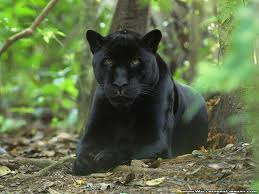
\includegraphics[scale=1, angle=0]{panther.jpg}
    \caption[The panther]{A panther is always watching}
    \label{fig: jordan}
\end{figure}

Duis nec quam quam, sed euismod justo. Pellentesque eu tellus vitae ante tempus malesuada. Nunc accumsan, quam in congue consequat, lectus lectus dapibus erat, id aliquet urna neque at massa. Nulla facilisi. Morbi ullamcorper eleifend posuere. Donec libero leo, faucibus nec bibendum at, mattis et urna. Proin consectetur, nunc ut imperdiet lobortis, magna neque tincidunt lectus, id iaculis nisi justo id nibh. Pellentesque vel sem in erat vulputate faucibus molestie ut lorem.


\begin{figure}
        \centering
        \begin{subfigure}[b]{0.4\textwidth}
                \centering        %   l   b   r   t
                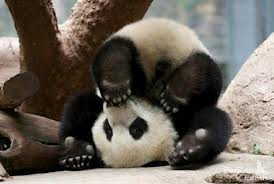
\includegraphics[trim=0.3cm 0cm 0cm 0cm, clip=true, 
                                width=\linewidth]
                                {panda.jpg}
                \caption{Panda}
                \label{subfig: ff}
        \end{subfigure}
        ~ % for a little horisontal distance
        \raisebox{3cm}[\height][\depth]{$\Rightarrow$}
        \hspace{0.2mm} % for a little horisontal distance
        \begin{subfigure}[b]{0.4\textwidth}
                \centering
                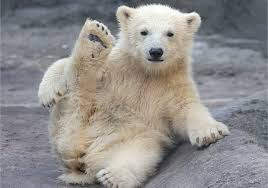
\includegraphics[trim=0cm 0cm 0cm 0cm, clip=true, 
                                width=\linewidth]
                                {polarbear.jpg}
                \caption{Polar bear}
                \label{subfig: sf}
        \end{subfigure}
        \caption[The panda-polar bear relationship ]
                {It is not widely known that the panda becomes a polar bear 
                when dressing up in the winter camouflage suite \cite{AnExpert}}
        \label{fig: pentagram}
\end{figure}




 % Background Theory 

%*******10********20********30********40********50********60********70********80

% For all chapters, use the newdefined chap{} instead of chapter{}
% This will make the text at the top-left of the page be the same as the chapter

\chap{Development Method}

Tables are good \cite{ATraveler} which is shown in \ref{table: you} and 
\ref{table: whether}!
\begin{table}[ht] 
    \centering 
    \begin{tabular}{|r|l|}
        \hline
        7C0 & hexadecimal \\
        3700 & octal \\ \cline{2-2}
        11111000000 & binary \\
        \hline \hline
        1984 & decimal \\
        \hline
    \end{tabular}
    \caption[You-table]{Table for you}
    \label{table: you} % is used to refer this table in the text 
\end{table} 

\begin{table}[ht] 
    \centering 
    \begin{tabular}{ | l | l | l | p{5cm} |}
        \hline
        Day & Min Temp & Max Temp & Summary \\ \hline
        Monday & 11C & 22C & A clear day with lots of sunshine. \\ \hline
        Tuesday & 9C & 19C & Cloudy with rain, \\ \hline
        Wednesday & 10C & 21C & Rain will still linger for the morning.\\
        \hline
    \end{tabular}
    \caption[Weather table]{Whether table for tomorrow}
    \label{table: whether} 
\end{table} 


 % Experimental Setup

%\input{Chapters/Chapter4} % Experiment 1

%\input{Chapters/Chapter5} % Experiment 2

%\input{Chapters/Chapter6} % Results and Discussion

%\input{Chapters/Chapter7} % Conclusion



%% Appendices -----------------------------------------------------
\addtocontents{toc}{\vspace{2em}} % Add a gap in the Contents, for aesthetics
\lhead{\emph{appendices}}  % Change the left side page header to "Appendices"
\appendix % Cue to tell LaTeX that the following 'chapters' are Appendices

\chap{An Appendix}

Lorem ipsum dolor sit amet, consectetur adipiscing elit. Vivamus at pulvinar nisi. Phasellus hendrerit, diam placerat interdum iaculis, mauris justo cursus risus, in viverra purus eros at ligula. Ut metus justo, consequat a tristique posuere, laoreet nec nibh. Etiam et scelerisque mauris. Phasellus vel massa magna. Ut non neque id tortor pharetra bibendum vitae sit amet nisi. Duis nec quam quam, sed euismod justo. Pellentesque eu tellus vitae ante tempus malesuada. Nunc accumsan, quam in congue consequat, lectus lectus dapibus erat, id aliquet urna neque at massa. Nulla facilisi. Morbi ullamcorper eleifend posuere. Donec libero leo, faucibus nec bibendum at, mattis et urna. Proin consectetur, nunc ut imperdiet lobortis, magna neque tincidunt lectus, id iaculis nisi justo id nibh. Pellentesque vel sem in erat vulputate faucibus molestie ut lorem.

Quisque tristique urna in lorem laoreet at laoreet quam congue. Donec dolor turpis, blandit non imperdiet aliquet, blandit et felis. In lorem nisi, pretium sit amet vestibulum sed, tempus et sem. Proin non ante turpis. Nulla imperdiet fringilla convallis. Vivamus vel bibendum nisl. Pellentesque justo lectus, molestie vel luctus sed, lobortis in libero. Nulla facilisi. Aliquam erat volutpat. Suspendisse vitae nunc nunc. Sed aliquet est suscipit sapien rhoncus non adipiscing nibh consequat. Aliquam metus urna, faucibus eu vulputate non, luctus eu justo.

Donec urna leo, vulputate vitae porta eu, vehicula blandit libero. Phasellus eget massa et leo condimentum mollis. Nullam molestie, justo at pellentesque vulputate, sapien velit ornare diam, nec gravida lacus augue non diam. Integer mattis lacus id libero ultrices sit amet mollis neque molestie. Integer ut leo eget mi volutpat congue. Vivamus sodales, turpis id venenatis placerat, tellus purus adipiscing magna, eu aliquam nibh dolor id nibh. Pellentesque habitant morbi tristique senectus et netus et malesuada fames ac turpis egestas. Sed cursus convallis quam nec vehicula. Sed vulputate neque eget odio fringilla ac sodales urna feugiat.

Phasellus nisi quam, volutpat non ullamcorper eget, congue fringilla leo. Cras et erat et nibh placerat commodo id ornare est. Nulla facilisi. Aenean pulvinar scelerisque eros eget interdum. Nunc pulvinar magna ut felis varius in hendrerit dolor accumsan. Nunc pellentesque magna quis magna bibendum non laoreet erat tincidunt. Nulla facilisi.

Duis eget massa sem, gravida interdum ipsum. Nulla nunc nisl, hendrerit sit amet commodo vel, varius id tellus. Lorem ipsum dolor sit amet, consectetur adipiscing elit. Nunc ac dolor est. Suspendisse ultrices tincidunt metus eget accumsan. Nullam facilisis, justo vitae convallis sollicitudin, eros augue malesuada metus, nec sagittis diam nibh ut sapien. Duis blandit lectus vitae lorem aliquam nec euismod nisi volutpat. Vestibulum ornare dictum tortor, at faucibus justo tempor non. Nulla facilisi. Cras non massa nunc, eget euismod purus. Nunc metus ipsum, euismod a consectetur vel, hendrerit nec nunc. % Appendix Title

%\input{Appendices/AppendixB} % Appendix Title

%\input{Appendices/AppendixC} % Appendix Title


%% Bibliography ---------------------------------------------------
\backmatter % Cue to tell LaTeX that the following 'chapters' are Bibliography
\label{Bibliography}
\lhead{\emph{Bibliography}}  % left side page header to "Bibliography"
\bibliographystyle{unsrtnat}  % Use the "unsrtnat" BibTeX style for formatting the Bibliography

\begingroup
    \raggedright
    \sloppy
    \bibliography{bibliography}  % The references (bibliography) information are stored in the file named "Bibliography.bib"
\endgroup 


\end{document}  % The End
%% ----------------------------------------------------------------